\chapter{Introduction}
\indent Since the creation and adoption of cars in the early 1900s, people have sought to create autonomous, or self-driving, cars. While early work proved to have little practical application or success, improvements to machine learning and artificial intelligence has once again reignited the push for self-driving cars. Companies such as Google and Tesla have already begun to mobilize self-driving cars proving that the technology for self-driving cars is rapidly improving \cite{dormehl_edelstein_2018}. However, while the technology to drive these cars have begun to slowly solidify, a few problems still linger. One such problem this paper will discuss is the visibility of data and memory consumption need for the cars to drive effectively.

\section{Data Gathering}

\indent Currently, most self-driving cars use 3D image segmentation to drive around. They gather data about the environment through a point cloud, which is a set of data points in three dimensional space. These point clouds can be collected through videos and more recently with the use of LIDAR (Light Detection and Ranging). LIDAR works by sending out a pulsed laser and using the feedback from the laser bouncing back to record distances and by combining this with video, creates a point cloud \cite{gisgeography_2018}. While point clouds can theoretically be small and sparse, most point clouds are quite dense as more data allows for better decision-making and thus better driving that a computer can do. As such, LIDARs produce very dense point clouds and can send around 160,000 pulses of light from the laser per second.

\section{Memory Consumption}

\indent This brings about the caveat of point clouds, which is that they take up large amounts of memory. For example, \ref{fig:pointCloud1} shows a point cloud consisting of 44,574,647 points with a memory size of ~1.6 GB compared to the image of the point cloud which has a memory size of ~3 MB \cite{schauer_2017}. This can cause problems for self-driving cars when they save the point clouds for processing or need to output to humans what the car sees. One example is with new scenarios a self-driving car may encounter. Currently, self-driving cars are able to distinguish most common scenes and scenarios, but it is still hard for self-driving cars to understand every situation that they comes across. As a result, human interaction may still be required in some instances to decipher problems a self-driving car may encounter. In these situations, it is not optimal for a person to take a look at a point cloud of what the car sees due to the requirement of a very dense point cloud for the point cloud to look realistic. 

\begin{figure}
  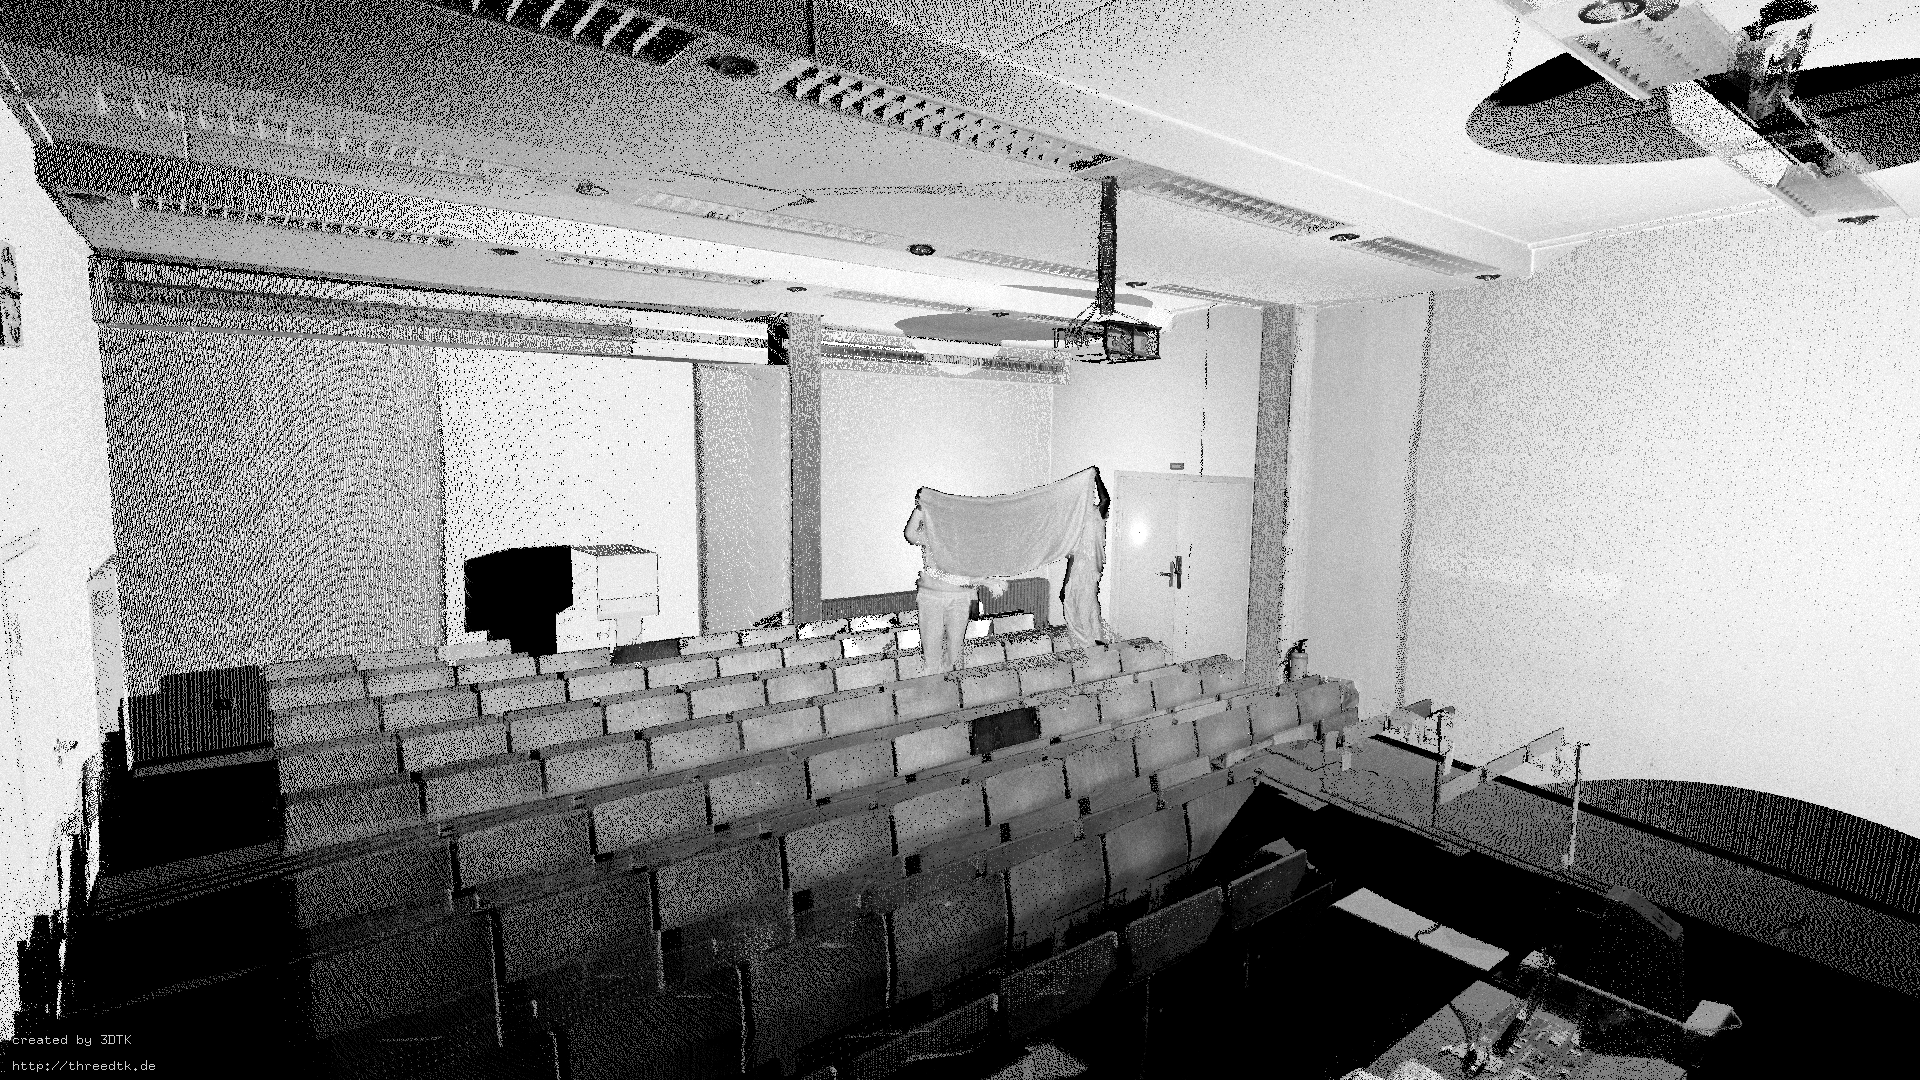
\includegraphics[width=\linewidth]{figures/lecturehall1.png}
  \caption{Example Point Cloud of a Lecture Room \cite{schauer_2017}}
  \label{fig:pointCloud1}
\end{figure}

\section{Contribution}

\indent A solution to these types of problems would be to segment the point cloud and identify the different objects in the point cloud. From there, the segmented points would be replaced with low-poly predefined geometric models (e.g. car model, street light model, building model) so that the object would be comprised of less points while still having the same amount of data that the computer needs. In addition, the segmentation and introduction of models cause the data to be simpler to process by the computer, improving the processing speed of the data. The models also give people a better image of what the car sees. In this work, I will implement this solution to take in a video and LIDAR point cloud and segment the video. From the segmented video, the program will replace each segmented object with the low-poly geometric models creating a 3D world that a user can look around in to see what a car is seeing.
